\section{Metodologia}
\label{gestio:metodologia}
Al llarg d'aquesta secció es tractaran mecàniques de funcionament i desenvolupament, funcionament d'equip, mètodes de validació, etc.
\subsection{Organització de l'equip}
\label{metodologia:oranitzacio_equip}
Al tractar-se d'un projecte realitzat en una empresa, conjuntament amb l'equip de desenvolupadors d'aquesta, el més normal és que s'adopti la manera de funcionar i organitzar-se de l'equip.\\
En aquest cas concret, la forma d'organització és mitjançant \textit{Scrum}.\\
\newline \textit{Scrum} és, de les conegudes com ``metodologies àgils'' la de més renom i provada eficàcia. Alhora, donada la tipologia de l'equip, sovint es fa ús de la coneguda com \textit{Kanban}, però sense oblidar les bondats d'\textit{scrum}.\\
\newline Per una banda, \textit{scrum} planteja un funcionament a base d'iteracions (\textit{sprints}) generalment de dues o quatre setmanes on al principi de cada una d'aquestes iteracions es manté una reunió (\textit{Sprint Planning Meeting}) on es busca planificar les tasques a desenvolupar al llarg de l'\textit{sprint} que comença el mateix dia de la reunió.
\begin{figure}[h]
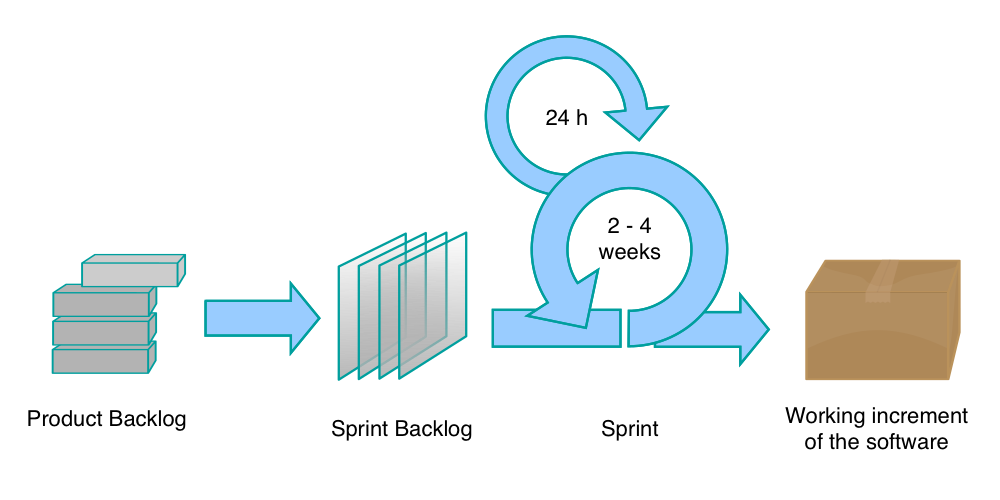
\includegraphics[scale=0.4]{sections/gestio/scrum_process.png}
\centering
\caption{Scrum}
\label{fig:scrum}
\end{figure}
\newline De la mateixa manera, \textit{scrum} proposa un seguit de reunions diàries on cada un dels membres de l'equip ha de respondre les següents preguntes:
\begin{itemize}
	\item Què es va fer ahir?
	\item Què es farà avui?
	\item Quins impediments s'han trobat fins ara?
\end{itemize}
El simple fet de respondre les anteriors preguntes, dóna als membres de l'equip una visió global de l'estat actual del projecte i permet intentar buscar solucions als entrebancs que puguin sorgir d'una forma col·laborativa on cada desenvolupador pot aportar el seu punt de vista i possibles solucions.\\
\newline Alhora, aquestes reunions permeten identificar desviacions del projecte i trobar-hi la solució adient abans de que el problema afecti de forma real, al global del projecte.\\
\newline \textit{Kanban} pel seu costat planteja l'acumulació de totes les tasques a desenvolupar en un mateix \textit{dashboard} visible per a tots els membres de l'equip organitzat en tres columnes:
\begin{itemize}
    \item \textit{ToDo}: on s'acumulen totes les tasques en el realitzar al projecte.
    \item \textit{Doing}: passen a aquesta columna només les que cada desenvolupador està realitzant en aquell moment.
    \item \textit{Done}: on s'acumulen les tasques ja finalitzades.
\end{itemize}
A mesura que avança el projecte, la idea és que cada desenvolupador agafi tasques de la columna \textit{ToDo} i les vagi passant a la columna \textit{Done}.\\
\newline Així doncs, en el cas concret d'aquest projecte, la dinàmica de l'equip ha estat la de fer ús de \textit{kanban} i el seu \textit{dashboard} de tres columnes, sense renunciar a la bondat de les \textit{daylies} que proposa \textit{scrum}.\\
\newline Aquesta barreja de metodologies ha permès detectar problemes i solucionar-los a temps, tal i com es veurà posteriorment al llarg de la secció \namref{desenvolupament}.
%Per al desenvolupament del projecte s'adoptaran les metodologies emprades a l'empresa, que en aquest cas, són el que s'anomenen metodologies àgils; concretament l'anomenada \textit{Scrum}\cite{scrum}.\\
%\\\textit{Scrum} es basa en la realització d'iteracions durant el procés de desenvolupament que reven el nom d'\textit{sprints}. Les esmentades iteracions es composen d'un seguit de tasques que s'han de completar al llarg de la durada dels \textit{sprints}; que acostuma a oscil·lar entre una setmana i un mes.\\
%\\Els objectius a assolir durant l'\textit{sprint} es fixen en unes reunions que es duen a terme a l'inici anomenades \textit{Sprint Planning Meeting}.\\
%Per altra banda, durant l'exercici de l'\textit{sprint} es realitzen reunions periòdiques anomenades \textit{Daily Scrum Meetings}, on es tracta de respondre a les següents preguntes:
%\begin{itemize}
%	\item Què es va fer ahir?
%	\item Què es farà avui?
%	\item Quins impediments s'han trobat fins ara?
%\end{itemize}
%Les anteriors preguntes intenten donar una visió el més àmplia possible de l'estat del projecte a tots els memebres de l'equip, així com permetre la resolució col·laborativa dels diferents problemes que vagin apareixent al llarg del desenvolupament.\\
%\\\textit{Scrum} permet reaccionar de forma àgil a les diferents alteracions que poden sorgir al llarg del desenvolupament i que els desenvolupadors realitzin els canvis pertinents.\\
%\\Al tractar-se d'un equip de desenvolupament reduït on la comunicació entre membres és constant, el seguiment de la filosofia \textit{scrum} resulta a vegadas un tant òbvia. Tot i aixó, es respecten les \textit{daylies} a l'inici de cada jornada i els \textit{sprint plannings} a l'inici de cada iteració.
\subsection{Codi i control de versions}
\label{metodologia:codi_versions}
Per al control de versions del projecte, es fa ús de repositoris \textit{git}\footnote{https://git-scm.com/}, un repositori destinat al \textit{frontend} i un per al \textit{backend}.\\
\newline Els repositoris estan estructurats tal i com s'indica a \textit{gitflow}\footnote{http://nvie.com/posts/a-successful-git-branching-model/}, una estandarització per a l'ús de branques a repositoris principalment git.\\
\begin{figure}[h]
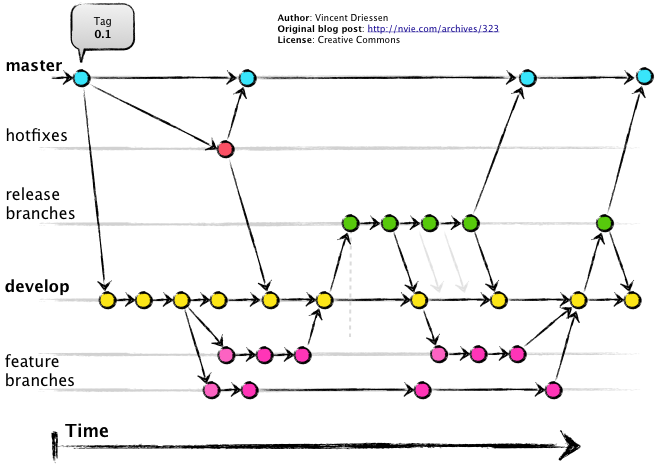
\includegraphics[scale=0.5]{sections/gestio/gitflow.png}
\centering
\caption{Gitflow}
\label{fig:gitflow}
\end{figure}
\clearpage
Internament els repositoris segueixen l'estructura mostrada a la Figura \ref{fig:gitflow}).\\
En essència es pot resumir l'esquema anterior en un repositori amb dues branques principals:
\begin{itemize}
	\item \textbf{Master}: En aquesta branca només hi ha codi plenament funcional i testejat. El codi que aquí es troba, està preparat per a ser publicat en qualsevol moment.
	\item \textbf{Develop}: La branca de desenvolupament. El codi que aquí es trobi, també haurà d'estar testejat i ésser funcional, però el grau de rigurositat d'aquesta branca és menor que a \textit{master}.
\end{itemize}
Partint d'aquestes branques inicials, a mesura que avanci el projecte es creuran noves branques a partir de la branca \textit{develop}, mai desde \textit{master}. A \textit{master} només s'hi passarà el codi que des de la branca \textit{develop} es consideri apte.\\
\newline Les branques es crearan a partir de les tasques definides a la secció \ref{gestio:tasques},
el nom de les branques ve donat pel programari de gestió de tasques que es fa servir (a la secció \nameref{metodologia:software_suport} es donen detalls del programari emprat), ja que d'aquesta forma queden vinculades les tasques amb els \textit{commits} i les branques.\\
\newline A nivell d'equip, les dinàmiques són senzilles.
\begin{itemize}
    \item Cada tasca en una branca.
    \item Un cop acabada la tasca, es porten els canvis cap a la branca \textit{develop}.
    \item En cas d'haver de solucionar errors sobre \textit{master} es farà creant branques amb el l'etiqueta \textit{bugfix}.
    \item Cada cop que una tasca es doni per finalitzada i validada, s'elimina la branca.
\end{itemize}
\subsubsection{TDD}
\label{metodologia:tdd}
Rep el nom de \textit{TDD}\footnote{Test-Driven Development} un conjunt de pràctiques de desenvolupament de programari que incideixen en la repetició, de forma reiterativa, d'un cicle de tres fases.
\begin{figure}[h]
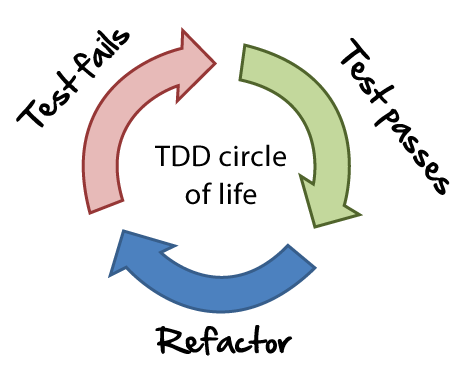
\includegraphics[scale=0.25]{sections/gestio/tdd_circle.png}
\centering
\caption{TDD}
\label{fig:tdd}
\end{figure}
\newline La figura anterior ens mostra el cicle de vida de \textit{TDD}, format per les tres fases anteriorment esmentades:
\begin{enumerate}
    \item Vermell, abans de la funcionalitat s'ha de desenvolupar el test i fer que falli
    \item Verd, es desenvolupa la funcionalitat i passa els testos
    \item Blau, refactoritzar el codi
\end{enumerate}
El seguir aquest \textit{workflow} té dos grans avantatges:
\begin{itemize}
    \item Primerament, el codi queda testejat, i es poden detectar errors en el comportament de cara  futurs canvis.
    \item Desenvolupar el test abans que la pròpia funcionalitat fa que mentalment el codi quedi estructurat i es contemplin casos d'ús, que normalment passarien per alt.
\end{itemize}
\subsection{Programari de suport}
\label{metodologia:software_suport}
Per a facilitar la gestió del projecte es disposa del programari de la suite \textit{Atlassian}\footnote{https://www.atlassian.com/}. En concret es fan servir:
\begin{itemize}
    \item \textit{Jira}, per a la gestió de tasques. Disposa de \textit{plugins} per \textit{kanban} i \textit{scrum}. A part, permet obtenir gràfics i lectures sobre l'activitat al repositori, tant individual com d'equip.
    \item \textit{Bitbucket}, com a repositori de git. Permet la creació de branques i realitzar operacions sobre els mateixos repositoris.
    \item \textit{Confluence}, l'espai on l'equip documenta qualsevol incidència o millores.
\end{itemize}
Addicionalment,també es fan servir clients d'escriptori de git per agilitzar les operacions del dia a dia amb el repositori.\\
\newline Per a la integració contínua es fa servir \textit{Jenkins}\footnote{https://jenkins.io/}. Un programari que permet desplegar els últims canvis del sistema, que hi hagi repositori de forma automàtica.
%Com a suport per a la gestió d'\textit{Scrum}\cite{scrum} i del control de versions, així com de documentació interna, es disposa de llicència de la suite d'\textit{Atlassian}\cite{atlassian}, que ofereix diferents aplicatius:
%\begin{itemize}
%	\item \textbf{Jira}: per a la gestió de tasques i planificació de les iteracions.
%	\item \textbf{Confluence}: per a la documentació interna del projecte.
%	\item \textbf{Bitbucket}: com a repositori de control de versions.
%\end{itemize}
%Per altra banda, també es fa servir \textit{Jenkins}\cite{jenkins} per a la integració contínua.
\subsection{Validació}
\label{metodologia:validacio}
%El mètode de validació que se segueix va lligat amb la metodologia \textit{Scrum}.\\
%\textit{Scrum}, defineix una serie d'iteracions a partir de les quals s'organitza la feina a realitzar al llarga de tot el projecte. En acabar cada una d'aquestes iteracions, per a que el codi sigui acceptat,  aquest ha de ser totalment funcional i presentar-se amb una bateria de tests que garantitzin el seu bon funcionament.
El mètode de validació que se segueix compleix dos criteris:
\begin{itemize}
    \item Compleix els requisits de la tasca
    \item La funcionalitat ha esta testejada adequadament.
\end{itemize}
Si es compleixen aquestes dos condicions, una de sentit comú, i l'altra donada per una de les metodologies de desenvolupament vistes anteriorment (\nameref{metodologia:tdd}), el codi es pot considerar apte.\\
El fet de tenir amb un codi testejat, assegura que si es fan canvis al codi es poden detectar canvis de comportament i errors fàcilment.


%\subsection{Organització de l'equip}
%Per al desenvolupmanet del projecte s'adoptaran les metodologies emprades a l'empresa, que en aquest cas, són el que s'anomenen metodologies àgils; concretament l'anomenada \textit{Scrum}\cite{scrum}.\\
%\textit{Scrum} es basa en la realització d'iteracions durant el procés de desenvolupament que reven el nom d'\textit{sprints}. Les esmentades iteracions es composen d'un seguit de tasques que s'han de completar al llarg de la durada dels \textit{sprints}; que acostuma a oscil·lar entre una setmana i un mes.\\
%Els objectius a assolir durant l'\textit{sprint} es fixen en unes reunions que es duen a terme a l'inici anomenades \textit{Sprint Planning Meeting}.\\
%Per altra banda, durant l'exercici de l'\textit{sprint} es realitzen reunions periòdiques anomenades \textit{Daily Scrum Meetings}, on es tracta de respondre a les següents preguntes:
%\begin{itemize}
%	\item Què vaig fer ahir?
%	\item Què faré avui?
%	\item Quins impediments he trobat fins ara?
%\end{itemize}
%Les anteriors preguntes intenten donar una visió el més àmplia possible de l'estat del projecte a tots els memebres de l'equip, així com permetre la resolució col·laborativa dels diferents problemes que vagin apareixent al llarg del desenvolupament.\\
%\textit{Scrum} permet reaccionar de forma àgil a les diferents alteracions que poden sorgir al llarg del desenvolupament i que els desenvolupadors realitzin els canvis pertinents.\\
%Al tractar-se d'un equip de desenvolupament reduït on la comunicació entre membres és constant, el seguiment de la filosofia \textit{scrum} resulta a vegadas un tant òbvia. Tot i aixó, es respecten les \textit{daylies} a l'inici de cada jornada i els \textit{sprint plannings} a l'inici de cada iteració.
%\subsection{Codi i control de versions}
%El desenvolupament del codi del projecte es divideix en dos parts clarament diferenciades:
%\begin{itemize}
%	\item \textbf{Backend}: desenvolupat amb Symfony, un dels frameworks PHP més extesos dins de la comunitat PHP per la seva versatilitat i potència.
%	\item \textbf{Frontend}: desenvolupat amb AngularJS, un framework suportat per Google i  que recentment ha alliberat la release final de la versió 2. Actualment, es postula com un dels principals frameworks 
%\end{itemize}
%Pel control de versions es fa ús de \textit{Git}\cite{git}, un sistema de control de versions desenvolupat primerament per Linus Torvalds (creador del kernel de Linux) i que gràcies a plataformes com \textit{GitHub} o \textit{Bitbucket} s'ha convertit en un dels sistemes de control de versions més emprat en el món del desenvolupament de software.\\
%\newline Per altra banda, per tal d'organitzar el flux de treball dins del repositori, s'ha decidit seguir un esquema com és \textit{Gitflow}\cite{gitflow}.\\
%A mode de resum, \textit{gitflow} proposa una organització dins del repositori molt clara i estructurada. \\
%\newpage
%L'estructura bàsica del repositori comptarà amb dos branques principals:
%\begin{itemize}
%	\item \textbf{Master}: en termes més autòctons, la branca de producció. En aquesta branca del repositori sols hi ha codi plenament funcional i testejat. El codi que aquí es troba, està preprat per a ser publicat en qualsevol moment.
%	\item \textbf{Develop}: aquesta és la branca que es destinarà al desenvolupament del codi pròpiament dit. El codi que aquí es trobi, també haurà d'estar testejat i ésser funcional, però el grau de rigurositat d'aquesta branca és menos que \textit{master}.
%\end{itemize}
%Un cop definit el punt de partida, es crearan branques a partir de la branca desenvolupament per a les diferents funcionalitats, aquestes rebran el nom de \textit{feature} seguit del codi de la tasca a desenvolupar. D'aquesta manera les branques queden etiquetades i vinculades amb la tasca.
%\newline Un cop acabada una tasca, es farà \textit{merge} de la branca \textit{feature-X} cap a la branca de desenvolupament i així successivament.
%\newline Un cop acabat l'\textit{sprint}, es farà \textit{merge} de la branca desenvolupament cap a la branca \textit{master}. Aquest procediment l'anomenarem \textit{release}.
%\newline Per a possibles correccions d'última hora, \textit{gitflow} proposa una quarta branca anomenada \textit{bugfix}. Aquesta surt directament de la branca \textit{master}, i està pensada per a correccions de codi ràpides.\\
%Per tal de mantenir el repositor el més net possible, cada cop que s'acabi una \textit{feature} o un \textit{bugfix} s'ha de tancar la branca creada.

%\subsection{Software de suport}
%Com a suport per a la gestió d'\textit{Scrum}\cite{scrum} i del control de versions, així com de documentació interna, es disposa de llicència de la suite d'\textit{Atlassian}\cite{atlassian}, que ofereix diferents aplicatius:
%\begin{itemize}
%	\item \textbf{Jira}: per a la gestió de tasques i planificació de les iteracions.
%	\item \textbf{Confluence}: per a la documentació interna del projecte.
%	\item \textbf{Bitbucket}: com a repositori de control de versions.
%\end{itemize}
%Per altra banda, també es fa servir \textit{Jenkins}\cite{jenkins} per a la integració contínua.

%\subsection{Validació}
%El mètode de validació que se segueix va lligat amb la metodologia \textit{Scrum}.\\
%\textit{Scrum}, defineix una serie d'iteracions a partir de les quals s'organitza la feina a realitzar al llarga de tot el projecte. En acabar cada una d'aquestes iteracions, per a que el codi sigui acceptat,  aquest ha de ser totalment funcional i presentar-se amb una bateria de tests que garantitzin el seu bon funcionament.
